\documentclass[tikz, 11pt]{standalone}

\usepackage{tikz}
\usetikzlibrary{shapes.geometric, arrows.meta, calc, decorations.pathmorphing}

\newcommand{\unit}{*2mm}
\newcommand{\arrow}{{Latex[length=1\unit, width=2\unit]}}
\newcommand{\lineWidth}{2pt}

\newcommand{\clockRadius}{10mm}
\newcommand{\hourHand}{5mm}
\newcommand{\minuteHand}{7mm}
\newcommand{\tickLength}{2mm}
\newcommand{\degOffset}{30}
\newcommand{\plugRadius}{2mm}
\newcommand{\plugLeg}{1.5mm}
\newcommand{\barWidth}{4mm}
\newcommand{\barHeight}{10mm}

% Styles
\tikzstyle{panel}=[draw=none, inner sep=0, outer sep=0]
\tikzstyle{bar}=[panel, fill=gray!50!white, minimum width=\barWidth, minimum height=\barHeight, rounded corners=0mm, draw=none, line width=\lineWidth]
\tikzstyle{line}=[draw=black, line width=\lineWidth, cap=round]
\tikzstyle{lineShort}=[line, shorten > =3mm, shorten < =3mm]
\tikzstyle{lines}=[line, rounded corners=1mm]
\tikzstyle{linesShort}=[lineShort, rounded corners=1mm]
\tikzstyle{arrow}=[line, -\arrow]
\tikzstyle{arrowShort}=[lineShort, -\arrow]
\tikzstyle{textNode}=[draw=none, inner sep=1mm]
\tikzstyle{textLabel}=[draw=none, inner sep=0, outer sep=0, text height=7pt, text depth=2pt]

\begin{document}

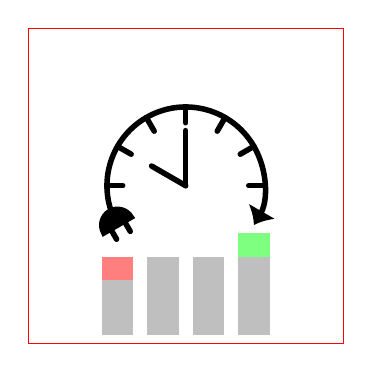
\begin{tikzpicture}[]

% Frame
\node[panel, draw=red, minimum width=4cm, minimum height=4cm] (frame) at (0,0) {};

% Useful coordinates
\coordinate (clockStart) at (180+\degOffset:\clockRadius);
\coordinate (clockEnd) at (-\degOffset:\clockRadius);

% Clock circle
\draw[arrow] 
  (clockStart) arc 
  (180+\degOffset:-\degOffset:\clockRadius); 
% Hands
\draw[line] (0,0) -- (150:\hourHand);
\draw[line] (0,0) -- (90:\minuteHand);
% Ticks
\foreach \a in {0,30,...,180} {
  \draw[line] (\a:\clockRadius-\tickLength) --(\a:\clockRadius);
  }
% Plug
\begin{scope}[rotate=\degOffset]
  \draw[line, fill=black] ($(clockStart)+(-\plugRadius, 0)$)
        arc[start angle=180, end angle=0, radius=\plugRadius] -- cycle;
  \draw[line] ($(clockStart)+(-0.5*\plugRadius, 0)$) --++ (0, -\plugLeg);
  \draw[line] ($(clockStart)+(0.5*\plugRadius, 0)$) --++ (0, -\plugLeg);
\end{scope}

\node[bar, anchor=north, fill=red, opacity=0.5, yshift=-4mm, minimum height=3mm] (barRemove) at (clockStart) {};
\node[bar, anchor=north, minimum height=7mm] (barLeft) at (barRemove.south) {};
\node[bar, anchor=north, yshift=-4mm] (barRight) at (clockEnd) {};
\node[bar, anchor=south, fill=green, opacity=0.5, minimum height=3mm] (barAdd) at (barRight.north) {};
\node[bar, anchor=south] at ($(barLeft.south)!1/3!(barRight.south)$) {};
\node[bar, anchor=south] at ($(barLeft.south)!2/3!(barRight.south)$) {};

\end{tikzpicture}
\end{document}